\documentclass[12pt,a4paper]{article}
\usepackage[utf8]{vietnam}
\usepackage{amsmath,amssymb}
\usepackage{tabularx}
\usepackage{graphicx}
\usepackage{tikz}
\usetikzlibrary{calc,arrows.meta}
\usepackage{xcolor}
\usepackage{enumitem}
\usepackage{fancyhdr}
\usepackage[top=1.0cm, bottom=1.0cm, left=1.3cm, right=1.3cm]{geometry}
\usepackage[loigiai]{ex_test}
\SAOPTN{widthSA=2.6,heightSA=0.62}

\setlength{\headheight}{15pt}
\setlength{\parskip}{1pt}

\pagestyle{fancy}
\fancyhf{}
\rhead{\textit{Lời giải chi tiết -- Đề số 10}}
\lhead{\textit{Bộ đề ôn tập Giữa học kì I -- Toán 7}}
\cfoot{\thepage}

\begin{document}

\begin{center}
\textbf{\Large HƯỚNG DẪN CHẤM VÀ LỜI GIẢI CHI TIẾT}\\
\vspace{1mm}
\textbf{\large MÔN: TOÁN 7 -- ĐỀ SỐ 10}
\end{center}
\vspace{2mm}

\noindent\textbf{\large PHẦN I. CÂU TRẮC NGHIỆM NHIỀU PHƯƠNG ÁN LỰA CHỌN}

\vspace{1mm}
\begin{ex}
Số nào dưới đây là số thập phân vô hạn tuần hoàn?
\choice
{$\dfrac{1}{2}$}
{$0{,}123123$}
{\True $0{,}(3)$}
{$0{,}3$}
\loigiai{
Số $0{,}(3) = 0{,}333\ldots$ là số thập phân vô hạn tuần hoàn với chu kỳ $3$.
}
\end{ex}

\begin{ex}
\immini{
Điểm $A$ trên trục số ở hình bên biểu diễn số hữu tỉ nào?
\choice
{$-\dfrac{2}{3}$}
{$\dfrac{1}{3}$}
{\True $\dfrac{2}{3}$}
{$\dfrac{4}{3}$}
}{
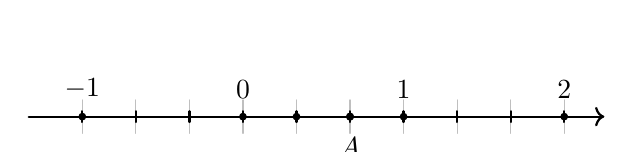
\begin{tikzpicture}[scale=0.85, line cap=round, line join=round]
    \draw[thick, ->] (-3.2, 0) -- (5.4, 0);
    \foreach \x in {-2.4, -1.6, -0.8, 0, 0.8, 1.6, 2.4, 3.2, 4.0, 4.8} {
        \draw[gray!50] (\x, -0.25) -- (\x, 0.25);
        \draw[thick] (\x, 0.08) -- (\x, -0.08);
    }
    \node[above=3pt] at (-2.4, 0) {$-1$};
    \node[above=3pt] at (0, 0) {$0$};
    \node[above=3pt] at (2.4, 0) {$1$};
    \node[above=3pt] at (4.8, 0) {$2$};
    \filldraw[black] (-2.4, 0) circle (1.4pt);
    \filldraw[black] (0, 0) circle (1.4pt);
    \filldraw[black] (0.8, 0) circle (1.4pt);
    \filldraw[black] (1.6, 0) circle (1.5pt) node[below=4pt, font=\bfseries] {$A$};
    \filldraw[black] (2.4, 0) circle (1.4pt);
    \filldraw[black] (4.8, 0) circle (1.4pt);
\end{tikzpicture}
}
\loigiai{
Đoạn đơn vị từ $0$ đến $1$ được chia thành $3$ phần bằng nhau. Điểm $A$ nằm ở vạch chia thứ hai theo chiều dương tính từ điểm gốc $0$ nên biểu diễn số hữu tỉ $\dfrac{2}{3}$.
}
\end{ex}

\begin{ex}
\immini{
Đọc tên các tia phân giác trong hình vẽ sau:
\choice
{$AB, BE$ là các tia phân giác}
{$AD, BC$ là các tia phân giác}
{\True $AD, BE$ là các tia phân giác}
{$AD, AB$ là các tia phân giác}
}{
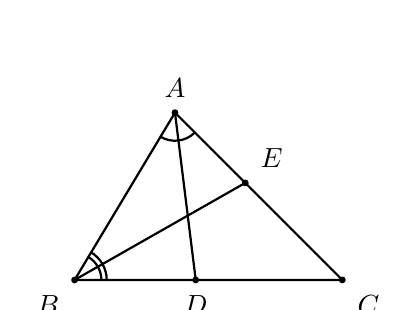
\begin{tikzpicture}[scale=0.85, line cap=round, line join=round]
    \coordinate (B) at (0, 0);
    \coordinate (C) at (4.0, 0);
    \coordinate (A) at (1.5, 2.5);
    \coordinate (D) at (1.81, 0);
    \coordinate (E) at (2.55, 1.45);

    \draw[thick] (A) -- (B) -- (C) -- cycle;
    \draw[thick] (A) -- (D);
    \draw[thick] (B) -- (E);

    \filldraw[black] (A) circle (1.2pt) node[above=2pt] {$A$};
    \filldraw[black] (B) circle (1.2pt) node[below left=2pt] {$B$};
    \filldraw[black] (C) circle (1.2pt) node[below right=2pt] {$C$};
    \filldraw[black] (D) circle (1.2pt) node[below=2pt] {$D$};
    \filldraw[black] (E) circle (1.2pt) node[above right=2pt] {$E$};

    % Bisector arcs at A
    \draw[thick] (A) ++(-121:0.42) arc (-121:-83:0.42);
    \draw[thick] (A) ++(-83:0.42) arc (-83:-45:0.42);
    % Bisector arcs at B
    \draw[thick] (B) ++(0:0.4) arc (0:29.5:0.4);
    \draw[thick] (B) ++(0:0.48) arc (0:29.5:0.48);
    \draw[thick] (B) ++(29.5:0.4) arc (29.5:59:0.4);
    \draw[thick] (B) ++(29.5:0.48) arc (29.5:59:0.48);
\end{tikzpicture}
}
\loigiai{
Ký hiệu trên hình cho thấy tia $AD$ chia góc $\widehat{BAC}$ thành hai góc bằng nhau và tia $BE$ chia góc $\widehat{ABC}$ thành hai góc bằng nhau. Do đó $AD, BE$ là các tia phân giác.
}
\end{ex}

\begin{ex}
Hình nào dưới đây là hình lăng trụ đứng tam giác?
\choice
{\True Hình có hai đáy là tam giác và ba mặt bên là hình chữ nhật}
{Hình có hai đáy là tứ giác và bốn mặt bên là hình chữ nhật}
{Hình có hai đáy là hình vuông và bốn mặt bên là hình vuông}
{Hình có một đáy là tam giác, một đỉnh chung}
\loigiai{
Theo định nghĩa, hình lăng trụ đứng tam giác có hai đáy là hình tam giác và ba mặt bên là các hình chữ nhật.
}
\end{ex}

\begin{ex}
Kết quả của phép tính $\left(-\dfrac{2}{5}\right)^2$ là:
\choice
{$-\dfrac{4}{25}$}
{\True $\dfrac{4}{25}$}
{$-\dfrac{2}{5}$}
{$\dfrac{4}{10}$}
\loigiai{
Áp dụng quy tắc tính lũy thừa của một phân số: $\left(-\dfrac{2}{5}\right)^2 = \dfrac{(-2)^2}{5^2} = \dfrac{4}{25}$.
}
\end{ex}

\begin{ex}
Số có thể viết dưới dạng số thập phân vô hạn tuần hoàn là:
\choice
{$\dfrac{3}{24}$}
{$-\dfrac{6}{25}$}
{\True $\dfrac{2}{15}$}
{$\dfrac{-5}{-8}$}
\loigiai{
Ta có $\dfrac{3}{24} = \dfrac{1}{8} = 0{,}125$; $-\dfrac{6}{25} = -0{,}24$; $\dfrac{-5}{-8} = \dfrac{5}{8} = 0{,}625$ là các số thập phân hữu hạn. Phân số tối giản $\dfrac{2}{15}$ có mẫu $15 = 3 \cdot 5$ chứa thừa số nguyên tố $3 \neq 2, 5$ nên viết được dưới dạng số thập phân vô hạn tuần hoàn.
}
\end{ex}

\begin{ex}
Giá trị của $x$ thỏa mãn $|x| = 3$ là:
\choice
{$x = 3$}
{$x = -3$}
{\True $x = 3$ hoặc $x = -3$}
{$x = 9$}
\loigiai{
Giá trị tuyệt đối của một số bằng $3$ khi số đó bằng $3$ hoặc bằng $-3$.
}
\end{ex}

\begin{ex}
\immini{
Cho hình vẽ bên, cần thêm điều kiện gì thì $AB \parallel DC$?
\choice
{$\widehat{BCD} = 60^\circ$}
{$\widehat{BCD} = 120^\circ$}
{$\widehat{BAD} = 60^\circ$}
{\True $\widehat{xAB} = 60^\circ$}
}{
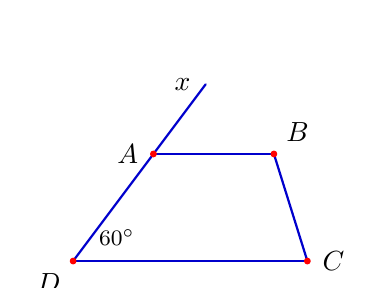
\begin{tikzpicture}[scale=0.85, line cap=round, line join=round]
    \coordinate (D) at (0, 0);
    \coordinate (C) at (3.5, 0);
    \coordinate (A) at (1.2, 1.6);
    \coordinate (B) at (3.0, 1.6);
    \coordinate (x) at ($(D)!1.65!(A)$);

    \draw[thick, blue!80!black] (D) -- (C);
    \draw[thick, blue!80!black] (A) -- (B);
    \draw[thick, blue!80!black] (B) -- (C);
    \draw[thick, blue!80!black] (D) -- (x);

    \filldraw[red] (A) circle (1.2pt) node[left=2pt, black] {$A$};
    \filldraw[red] (B) circle (1.2pt) node[above right=1pt, black] {$B$};
    \filldraw[red] (C) circle (1.2pt) node[right=2pt, black] {$C$};
    \filldraw[red] (D) circle (1.2pt) node[below left=1pt, black] {$D$};
    \node[left=2pt] at (x) {$x$};

    \node[font=\footnotesize, above right=1pt] at ($(D)+(0.2, 0.05)$) {$60^\circ$};
\end{tikzpicture}
}
\loigiai{
Hai đường thẳng $AB$ và $DC$ cùng cắt đường thẳng $Dx$. Hai góc $\widehat{xAB}$ và $\widehat{ADC}$ nằm ở vị trí đồng vị. Để $AB \parallel DC$ thì hai góc đồng vị phải bằng nhau, tức là $\widehat{xAB} = \widehat{ADC} = 60^\circ$.
}
\end{ex}

\begin{ex}
Hãy so sánh hai số hữu tỉ $-0{,}2$ và $\dfrac{-2}{5}$:
\choice
{$-0{,}2 < \dfrac{-2}{5}$}
{\True $-0{,}2 > \dfrac{-2}{5}$}
{$-0{,}2 = \dfrac{-2}{5}$}
{$-0{,}2 \ge \dfrac{-2}{5}$}
\loigiai{
Đổi $\dfrac{-2}{5} = -0{,}4$. Do $-0{,}2 > -0{,}4$ nên $-0{,}2 > \dfrac{-2}{5}$.
}
\end{ex}

\begin{ex}
Căn bậc hai số học của $49$ là:
\choice
{$-7$}
{\True $7$}
{$-7$ và $7$}
{$-49$}
\loigiai{
Căn bậc hai số học của $49$ là số không âm $x$ thỏa mãn $x^2 = 49$. Do $7 > 0$ và $7^2 = 49$ nên $\sqrt{49} = 7$.
}
\end{ex}

\begin{ex}
Qua một điểm $M$ nằm ngoài đường thẳng $a$, kẻ được bao nhiêu đường thẳng song song với đường thẳng $a$?
\choice
{Có vô số đường thẳng}
{Không có đường thẳng nào}
{Có hai đường thẳng}
{\True Chỉ có một đường thẳng}
\loigiai{
Theo tiên đề Euclid, qua một điểm nằm ngoài một đường thẳng chỉ có một đường thẳng song song với đường thẳng đó.
}
\end{ex}

\begin{ex}
Kết quả của phép tính $\dfrac{-3}{20} + \dfrac{-2}{15}$ là:
\choice
{$-\dfrac{1}{35}$}
{\True $-\dfrac{17}{60}$}
{$-\dfrac{5}{35}$}
{$-\dfrac{1}{60}$}
\loigiai{
Quy đồng mẫu số chung $60$: $\dfrac{-3}{20} + \dfrac{-2}{15} = \dfrac{-9}{60} + \dfrac{-8}{60} = -\dfrac{17}{60}$.
}
\end{ex}


\setcounter{ex}{0}
\noindent\textbf{\large PHẦN II. CÂU TRẮC NGHIỆM ĐÚNG SAI}

\vspace{1mm}
\begin{ex}
Cho biểu thức $A = \left(-\dfrac{1}{2}\right)^3 + \dfrac{3}{4} \cdot \left(-\dfrac{2}{3}\right) + \left|-\dfrac{5}{8}\right|$. Xét tính đúng sai của các mệnh đề sau:
\choiceTF
{\True Giá trị của lũy thừa $\left(-\dfrac{1}{2}\right)^3$ bằng $-\dfrac{1}{8}$}
{\True Giá trị của phép tính $\dfrac{3}{4} \cdot \left(-\dfrac{2}{3}\right)$ bằng $-\dfrac{1}{2}$}
{Giá trị tuyệt đối $\left|-\dfrac{5}{8}\right|$ bằng $-\dfrac{5}{8}$}
{\True Giá trị của biểu thức $A$ bằng $0$}
\loigiai{
\begin{itemize}[leftmargin=0.6cm, itemsep=1pt]
\item \textbf{a)} \textbf{Đúng}. Ta có $\left(-\dfrac{1}{2}\right)^3 = \left(-\dfrac{1}{2}\right) \cdot \left(-\dfrac{1}{2}\right) \cdot \left(-\dfrac{1}{2}\right) = -\dfrac{1}{8}$.
\item \textbf{b)} \textbf{Đúng}. Thực hiện phép nhân hai số hữu tỉ: $\dfrac{3}{4} \cdot \left(-\dfrac{2}{3}\right) = \dfrac{3 \cdot (-2)}{4 \cdot 3} = -\dfrac{2}{4} = -\dfrac{1}{2}$.
\item \textbf{c)} \textbf{Sai}. Giá trị tuyệt đối của một số luôn không âm, do đó $\left|-\dfrac{5}{8}\right| = \dfrac{5}{8}$.
\item \textbf{d)} \textbf{Đúng}. Thay các giá trị vừa tính vào biểu thức $A$ ta được: $A = -\dfrac{1}{8} + \left(-\dfrac{1}{2}\right) + \dfrac{5}{8} = -\dfrac{1}{8} - \dfrac{4}{8} + \dfrac{5}{8} = \dfrac{-1 - 4 + 5}{8} = 0$.
\end{itemize}
}
\end{ex}

\begin{ex}
\immini{
Quan sát hình vẽ bên, hai đường thẳng $xx'$ và $yy'$ cắt nhau tại điểm $O$. Biết số đo góc $\widehat{xOy} = 45^\circ$. Xét tính đúng sai của các mệnh đề sau:
\choiceTF
{\True Góc $\widehat{xOy}$ và góc $\widehat{x'Oy'}$ là hai góc đối đỉnh}
{\True Số đo của góc $\widehat{x'Oy'}$ bằng $45^\circ$}
{\True Góc $\widehat{xOy'}$ kề bù với góc $\widehat{xOy}$ và có số đo bằng $135^\circ$}
{Tổng số đo của hai góc đối đỉnh $\widehat{xOy}$ và $\widehat{x'Oy'}$ bằng $180^\circ$}
}{
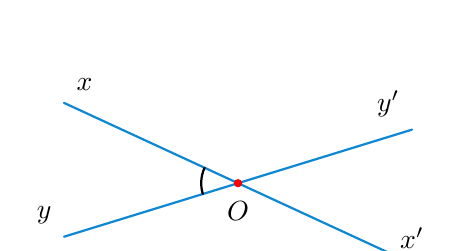
\begin{tikzpicture}[scale=0.85, line cap=round, line join=round]
    \coordinate (O) at (0, 0);
    \coordinate (x) at (-2.6, 1.2);
    \coordinate (x_prime) at (2.6, -1.2);
    \coordinate (y) at (-2.6, -0.8);
    \coordinate (y_prime) at (2.6, 0.8);

    \draw[thick, cyan!70!blue] (x) -- (x_prime);
    \draw[thick, cyan!70!blue] (y) -- (y_prime);

    \filldraw[red] (O) circle (1.5pt) node[below=3pt, black] {$O$};
    \node[above right=1pt] at (x) {$x$};
    \node[above=2pt] at (x_prime) {$x'$};
    \node[above left=1pt] at (y) {$y$};
    \node[above left=1pt] at (y_prime) {$y'$};

    % Arc for xOy
    \draw[thick] (O) ++(155.3:0.55) arc (155.3:197.1:0.55);
\end{tikzpicture}
}
\loigiai{
\begin{itemize}[leftmargin=0.6cm, itemsep=1pt]
\item \textbf{a)} \textbf{Đúng}. Tia $Ox'$ là tia đối của tia $Ox$ và tia $Oy'$ là tia đối của tia $Oy$, do đó hai góc $\widehat{xOy}$ và $\widehat{x'Oy'}$ nằm đối diện nhau qua đỉnh $O$ nên là hai góc đối đỉnh.
\item \textbf{b)} \textbf{Đúng}. Hai góc đối đỉnh thì bằng nhau, suy ra $\widehat{x'Oy'} = \widehat{xOy} = 45^\circ$.
\item \textbf{c)} \textbf{Đúng}. Hai góc $\widehat{xOy'}$ và $\widehat{xOy}$ có chung cạnh $Ox$ và hai cạnh $Oy, Oy'$ là hai tia đối nhau nên là hai góc kề bù. Số đo góc $\widehat{xOy'} = 180^\circ - \widehat{xOy} = 180^\circ - 45^\circ = 135^\circ$.
\item \textbf{d)} \textbf{Sai}. Tổng số đo của hai góc đối đỉnh này là $\widehat{xOy} + \widehat{x'Oy'} = 45^\circ + 45^\circ = 90^\circ \neq 180^\circ$.
\end{itemize}
}
\end{ex}


\setcounter{ex}{0}
\noindent\textbf{\large PHẦN III. CÂU HỎI TRẢ LỜI NGẮN}

\vspace{1mm}
\begin{ex}
Tìm số hữu tỉ $x$, biết: $\left(x - \dfrac{3}{4}\right)^2 = \dfrac{1}{16}$. \shortans{$x = 1$ hoặc $x = \dfrac{1}{2}$}
\loigiai{
Vì $\left(\dfrac{1}{4}\right)^2 = \dfrac{1}{16}$ và $\left(-\dfrac{1}{4}\right)^2 = \dfrac{1}{16}$ nên ta có hai trường hợp:
\begin{itemize}
    \item Trường hợp 1: $x - \dfrac{3}{4} = \dfrac{1}{4} \implies x = \dfrac{1}{4} + \dfrac{3}{4} = 1$.
    \item Trường hợp 2: $x - \dfrac{3}{4} = -\dfrac{1}{4} \implies x = -\dfrac{1}{4} + \dfrac{3}{4} = \dfrac{2}{4} = \dfrac{1}{2}$.
\end{itemize}
Vậy $x = 1$ hoặc $x = \dfrac{1}{2}$.

\textbf{Đáp số:} $x = 1$ hoặc $x = \dfrac{1}{2}$
}
\end{ex}

\begin{ex}
Cho góc $\widehat{mOn} = 140^\circ$, tia $Ot$ là tia phân giác của $\widehat{mOn}$. Tính số đo góc kề bù với góc $\widehat{mOt}$. \shortans{$110^\circ$}
\loigiai{
Vì $Ot$ là tia phân giác của góc $\widehat{mOn}$ nên:
\[ \widehat{mOt} = \dfrac{\widehat{mOn}}{2} = \dfrac{140^\circ}{2} = 70^\circ. \]
Góc kề bù với góc $\widehat{mOt}$ có số đo là: $180^\circ - 70^\circ = 110^\circ$.

\textbf{Đáp số:} $110^\circ$
}
\end{ex}


\setcounter{ex}{0}
\noindent\textbf{\large PHẦN IV. TỰ LUẬN}

\vspace{1mm}
\begin{ex}
Thực hiện phép tính:
\begin{enumerate}[label=\textbf{\alph*)}, leftmargin=0.8cm, itemsep=1pt]
\item $\dfrac{5}{12} + \left(-\dfrac{7}{24}\right) : \dfrac{3}{8}$;
\item $\dfrac{4}{5} \cdot \dfrac{3}{7} - \dfrac{-4}{7} : \sqrt{\dfrac{25}{16}} - |-1|$.
\end{enumerate}
\loigiai{
\textbf{a)} $\dfrac{5}{12} + \left(-\dfrac{7}{24}\right) : \dfrac{3}{8} = \dfrac{5}{12} + \left(-\dfrac{7}{24}\right) \cdot \dfrac{8}{3} = \dfrac{5}{12} + \left(-\dfrac{7}{9}\right) = \dfrac{15}{36} - \dfrac{28}{36} = -\dfrac{13}{36}$.

\textbf{b)} $\dfrac{4}{5} \cdot \dfrac{3}{7} - \dfrac{-4}{7} : \sqrt{\dfrac{25}{16}} - |-1| = \dfrac{12}{35} - \dfrac{-4}{7} : \dfrac{5}{4} - 1 = \dfrac{12}{35} - \dfrac{-4}{7} \cdot \dfrac{4}{5} - 1 = \dfrac{12}{35} - \left(-\dfrac{16}{35}\right) - 1 = \dfrac{12}{35} + \dfrac{16}{35} - 1 = \dfrac{28}{35} - 1 = \dfrac{4}{5} - 1 = -\dfrac{1}{5}$.
}
\end{ex}
\vspace{2mm}

\begin{ex}
Tìm $x$ biết:
\begin{enumerate}[label=\textbf{\alph*)}, leftmargin=0.8cm, itemsep=1pt]
\item $2x - \dfrac{1}{3} = \dfrac{5}{3}$;
\item $(2x + 3)^2 = 25$.
\end{enumerate}
\loigiai{
\textbf{a)} $2x - \dfrac{1}{3} = \dfrac{5}{3} \implies 2x = \dfrac{5}{3} + \dfrac{1}{3} = \dfrac{6}{3} = 2 \implies x = 2 : 2 = 1$. Vậy $x = 1$.

\textbf{b)} $(2x + 3)^2 = 25$. Vì $5^2 = 25$ và $(-5)^2 = 25$ nên ta có hai trường hợp:
\begin{itemize}
    \item TH 1: $2x + 3 = 5 \implies 2x = 2 \implies x = 1$.
    \item TH 2: $2x + 3 = -5 \implies 2x = -8 \implies x = -4$.
\end{itemize}
Vậy $x = 1$ hoặc $x = -4$.
}
\end{ex}
\vspace{2mm}

\begin{ex}
Một hồ bơi dạng hình hộp chữ nhật có kích thước là chiều dài $12\text{ m}$, chiều rộng $5\text{ m}$ và chiều sâu $3\text{ m}$.
\begin{enumerate}[label=\textbf{\alph*)}, leftmargin=0.8cm, itemsep=1pt]
\item Tính thể tích nước khi bể bơi đầy nước.
\item Người ta cần lát gạch bên trong lòng hồ (mặt đáy và bốn mặt xung quanh). Biết gạch hình vuông có cạnh $50\text{ cm}$. Hỏi cần mua ít nhất bao nhiêu viên gạch để lát bên trong lòng hồ bơi? (Coi diện tích mạch vữa lát không đáng kể).
\end{enumerate}
\loigiai{
\textbf{a)} Thể tích nước khi bể bơi đầy nước là:
\[ V = 12 \cdot 5 \cdot 3 = 180\text{ (m}^3\text{)}. \]

\textbf{b)} Diện tích xung quanh bên trong lòng hồ là:
\[ S_{xq} = 2 \cdot (12 + 5) \cdot 3 = 102\text{ (m}^2\text{)}. \]
Diện tích đáy hồ là:
\[ S_{\text{đáy}} = 12 \cdot 5 = 60\text{ (m}^2\text{)}. \]
Tổng diện tích cần lát gạch là:
\[ S = S_{xq} + S_{\text{đáy}} = 102 + 60 = 162\text{ (m}^2\text{)}. \]
Đổi $50\text{ cm} = 0{,}5\text{ m}$. Diện tích của một viên gạch là:
\[ S_{\text{gạch}} = 0{,}5 \cdot 0{,}5 = 0{,}25\text{ (m}^2\text{)}. \]
Số viên gạch ít nhất cần dùng là:
\[ 162 : 0{,}25 = 648\text{ (viên)}. \]
}
\end{ex}
\vspace{2mm}

\begin{ex}
Cho $A = \dfrac{1}{2^2} + \dfrac{1}{3^2} + \dfrac{1}{3^4} + \dfrac{1}{3^6} + \ldots + \dfrac{1}{3^{100}}$. Chứng minh rằng $A < \dfrac{3}{8}$.
\loigiai{
Ta tách biểu thức $A = \dfrac{1}{4} + B$, trong đó:
\[ B = \dfrac{1}{3^2} + \dfrac{1}{3^4} + \dfrac{1}{3^6} + \ldots + \dfrac{1}{3^{100}}. \]
Nhân cả hai vế của $B$ với $3^2 = 9$:
\[ 9B = 9 \cdot \left(\dfrac{1}{3^2} + \dfrac{1}{3^4} + \ldots + \dfrac{1}{3^{100}}\right) = 1 + \dfrac{1}{3^2} + \dfrac{1}{3^4} + \ldots + \dfrac{1}{3^{98}}. \]
Trừ từng vế $9B$ cho $B$:
\[ 9B - B = \left(1 + \dfrac{1}{3^2} + \ldots + \dfrac{1}{3^{98}}\right) - \left(\dfrac{1}{3^2} + \dfrac{1}{3^4} + \ldots + \dfrac{1}{3^{100}}\right) \]
\[ 8B = 1 - \dfrac{1}{3^{100}}. \]
Vì $\dfrac{1}{3^{100}} > 0$ nên $1 - \dfrac{1}{3^{100}} < 1$. Do đó $8B < 1 \implies B < \dfrac{1}{8}$.

Thay $B < \dfrac{1}{8}$ vào biểu thức $A$:
\[ A = \dfrac{1}{4} + B < \dfrac{1}{4} + \dfrac{1}{8} = \dfrac{2}{8} + \dfrac{1}{8} = \dfrac{3}{8}. \]
Vậy $A < \dfrac{3}{8}$.
}
\end{ex}
\vspace{2mm}


\begin{center}
\rule{4cm}{0.4pt}\\
\textit{--- HẾT ---}
\end{center}
\end{document}
